\documentclass[12pt]{article}
\usepackage{graphicx} % Required for inserting images
\usepackage[hidelinks]{hyperref}
\usepackage[style=apa,sortcites,backend=biber]{biblatex}
\usepackage{caption}

\title{Physical activity patterns as predictors of worsening depression}
\author{Author name redacted}
\date{December 2023}

\addbibresource{./ref.bib}

\begin{document}

\maketitle

\tableofcontents

\newpage

\section{Introduction}

This section of the report establishes the context of the connection between depression and physical activity and provides a condensed summary of the subsequent sections.

\subsection{Background}

Depression describes a common and widely prevalent family of mental disorders affecting an estimated $4.4\%$ of the global population \parencite{who}. Depression is commonly characterized by both physiological symptoms, such as fatigue, difficulties in concentrating and changes in appetite, psychological effects, including feelings of worthlessness and loss of interest in most activities, as well as behavioral changes, in particular, reduced physical activity \parencite{DSM5}. 
Among other factors, periods of decreased movement have been shown to be strongly associated with higher occurrence and severity of depressive episodes \parencite{O_Brien, Pinto, Harris}. While the direction of the causal relationship between active movement and expression of depressive symptoms is not definitively known and remains an area of active research, information about movement patterns offers valuable and comparatively accessible insight into one's psychological condition. The magnitude of the connection between depression and physical activity varies across different cohorts and observation methods, but the general trend of an inverse correlation between these two factors is reported by a substantial number of relevant studies \parencite{Parker_Brotchie_1992}. 

One of the methods of obtaining records of a person's movement is though the use of an actigraph — a wearable device equipped with an accelerometer that measures and records gross physical activity of the subject. Actigraphy has been gaining popularity in medical research since the 1980s, when precision and reliability of the accelerometer readings became sufficient for use in scientific studies \parencite{Berger_2008}. Since then, actigraphy has remained a valuable tool in studies of human behavior, including those focused on mental health and psychological disorders.


\subsection{Project summary}

For this study, we explored data collected during a 2010 study on motor activity of patients of a psychiatric hospital with the goal of understanding how movement data can be used to assist the diagnosis of depression and continued monitoring of the diagnosed patient's condition. The data set provides records of actigraph measurements collected from a group of subjects diagnosed with depression, along with similar data on a group of non-depressed subjects. The data is augmented with demographic information on the depressed subjects, as well as the results of a diagnostic questionnaire administered to each diagnosed subject before and after the study.

Our first objective was to replicate the experiments detailed in previous studies that explore the relationship between depression symptoms and physical activity. We aimed to verify the presence of an inverse correlation between the two. We then sought to uncover additional patterns in the activity of patients who have experienced worsening symptoms during the study, as compared to movement data of other patients and the control group.

We compared the movement behavior of the diagnosed patients to those of a healthy control group and concluded that depression is significantly correlated with reduced daytime physical activity within the studied populations. Further, we have analysed the activity patterns of patients who suffered worsening symptoms in comparison to the activity of symptomatically improving patients. By applying visualization techniques, we have uncovered that the worsening patients behave closer to the control group rather than other patients when it comes to afternoon and evening physical activity.

\section{Problem Formulation}

In this section we describe the area of research that we seek to contribute to and postulate the objectives we aim to accomplish with this project.

\subsection{Connection between activity and depression}

Before we examine the data set for novel research opportunities, it is important to verify that the patterns present in the data are consistent findings of previous studies. The association between the major depressive disorder and reduced physical activity has been firmly established in both case-control and longitudinal studies \parencite{Burton_2013}. Thus, if we discover that the examined data set presents evidence against the existing consensus, additional inquiry into this phenomena would be required.

\subsection{Activity of subjects with worsening depressive symptoms}

Our second and perhaps central objective is to evaluate the effectiveness of actigraphy in continuous patient monitoring after the initial depression diagnosis, particularly for the task of flagging patients with intensifying symptoms. Patients exhibiting adverse dynamic of their condition might be in need of most urgent help, which is why we have elected to focus specifically on this group.

While a variety of methods for regular evaluation of a patient's condition see wide use in psychology, many of them lack the precise, accessible, and unobtrusive measurement procedure offered by actigraphy. Should we uncover that movement observation through wearable devices is a technique suitable for continuous patient monitoring, we would be able to recommend further research into the use of wearables for this task.

As our objectives primarily relate to group observations, we have decided to forgo most of the individual level analysis in favor of a deeper dive into group-level patterns.

\section{Data Description}

This section describes the origin and contents of the data set used in the experiment and outlines the data processing methods used to prepare the data for exploration.

\subsection{Data set contents}

The data used for the present project was originally produced for a study on motor activity of patients suffering from depression and schizophrenia \parencite{Berle_2010}. The study provides records of gross physical activity of patients of a psychiatric ward at intervals of one minute over a period of 5-20 days. Records were obtained using an Actiwatch device worn on the right wrist, with each record presented as a numerical reading from the actigraph combined with a timestamp of the recording. In addition to movement data, the study also provides individual information on the subjects, with the information on the patients detailing gender, age group, education, marital status, employment, type of treatment (inpatient/outpatient), as well as some details of the depressive condition, including presence of melancholia and the type of affliction (unipolar, bipolar types 1 and 2). Crucially, two scorings on the Montgomery-Asberg (MADRS) scale \parencite{Montgomery_Asberg_1979} — one taken at the beginning of the study and one taken at its conclusion. Information on the control group subjects is limited to gender and age group. All variables mentioned above are of categorical nature, with the exception of the MADRS scores which take integer values in the interval between 0 and 60 points (higher score represents more severe symptoms).

In total, 23 subjects diagnosed with depression and an equal number of subjects suffering from schizophrenia were surveyed, in addition to 32 non-patient subjects who formed a control group. Within the scope of our study we do not consider data collected from patients with schizophrenia, focusing instead on data collected from patients with depression. We will refer to those patients as the \textit{condition group}.

\subsection{Prepossessing}

Before proceeding with exploring the data, we needed to complete several prepossessing and cleaning steps. Firstly, we need to decide on our approach to handling missing values. The table containing personal information on the patients harbored several empty cells, specifically in columns pertaining to education and melancholy. As these particular values were not crucial to our research, we elected to retain the rows with the missing data.

Secondly, for some of the patients, the actigraph data contained several blind spots, where movement data was missing for a certain period of time. After a brief investigation, we discovered that the intervals of the missing data were contained to one hour during the night of March 31st, which suggests that the perceived loss of data was likely caused by changing of the clock to the summer time and required no further action.

Finally, we suspected that the movement data could contain observations recorded during a time when the subject was not wearing their actigraph device. Such records have the potential of contaminating the experimental observations, particularly as we focus our attention on low activity days. To reduce the probability of contamination, we decided to filter away movement records during days of exceptionally low average activity. The cut-off threshold was initially set to a very low value, and was gradually increased until the observations close to the threshold began visually resembling believable daily activity records of a person and it was no longer possible to confidently classify those records as meaningless. An illustration comparing suspected meaningless data at the final threshold to meaningful observations is provided in Figure \ref{fig:sus}.

\begin{figure}[!h]
    \centering
    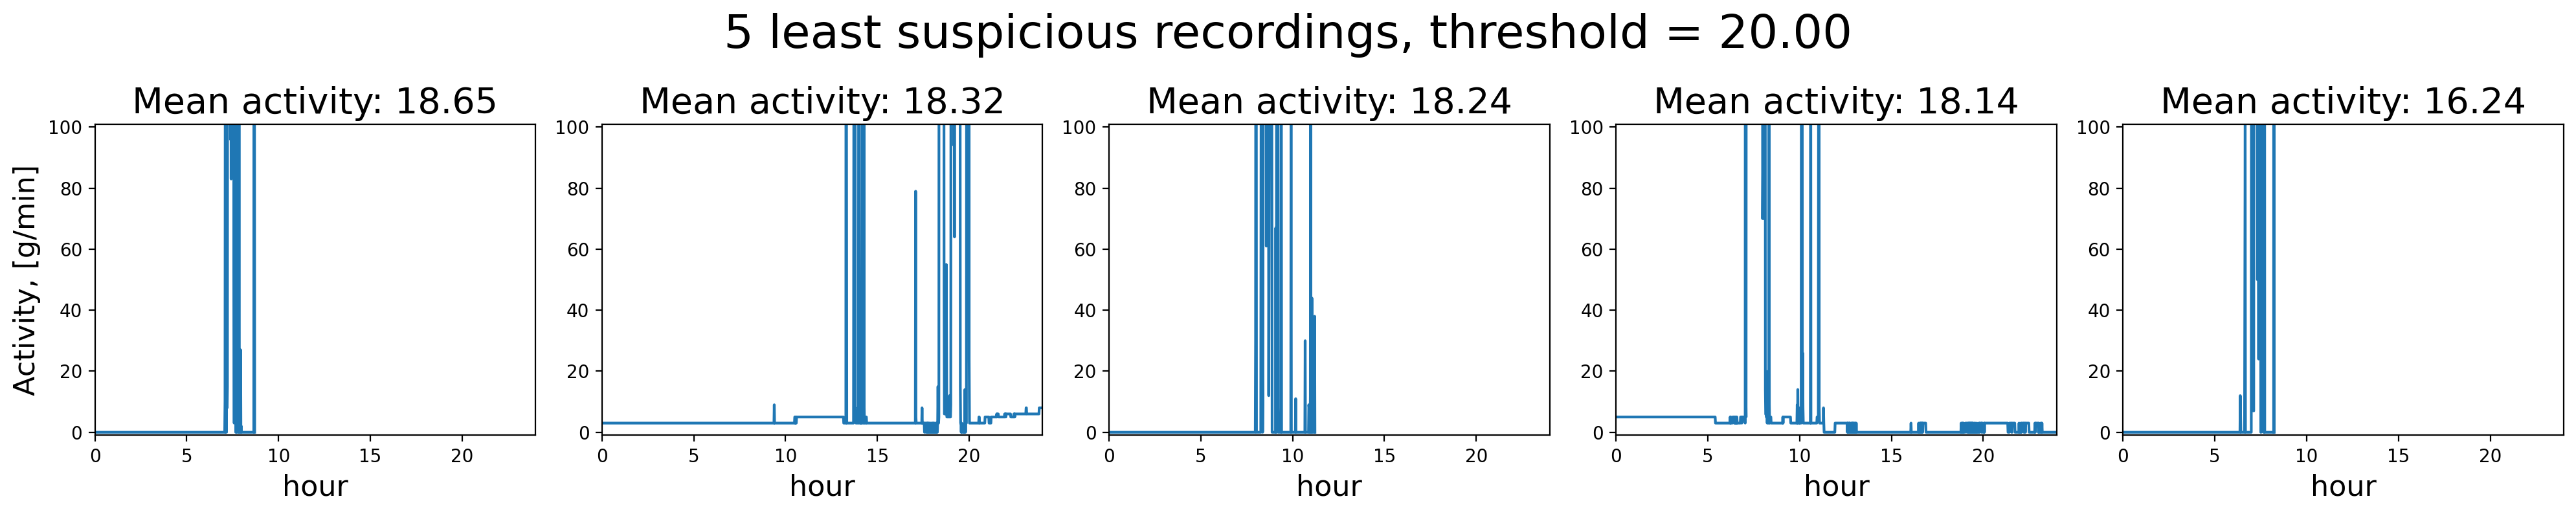
\includegraphics[width=.99\textwidth]{images/sus.png}
    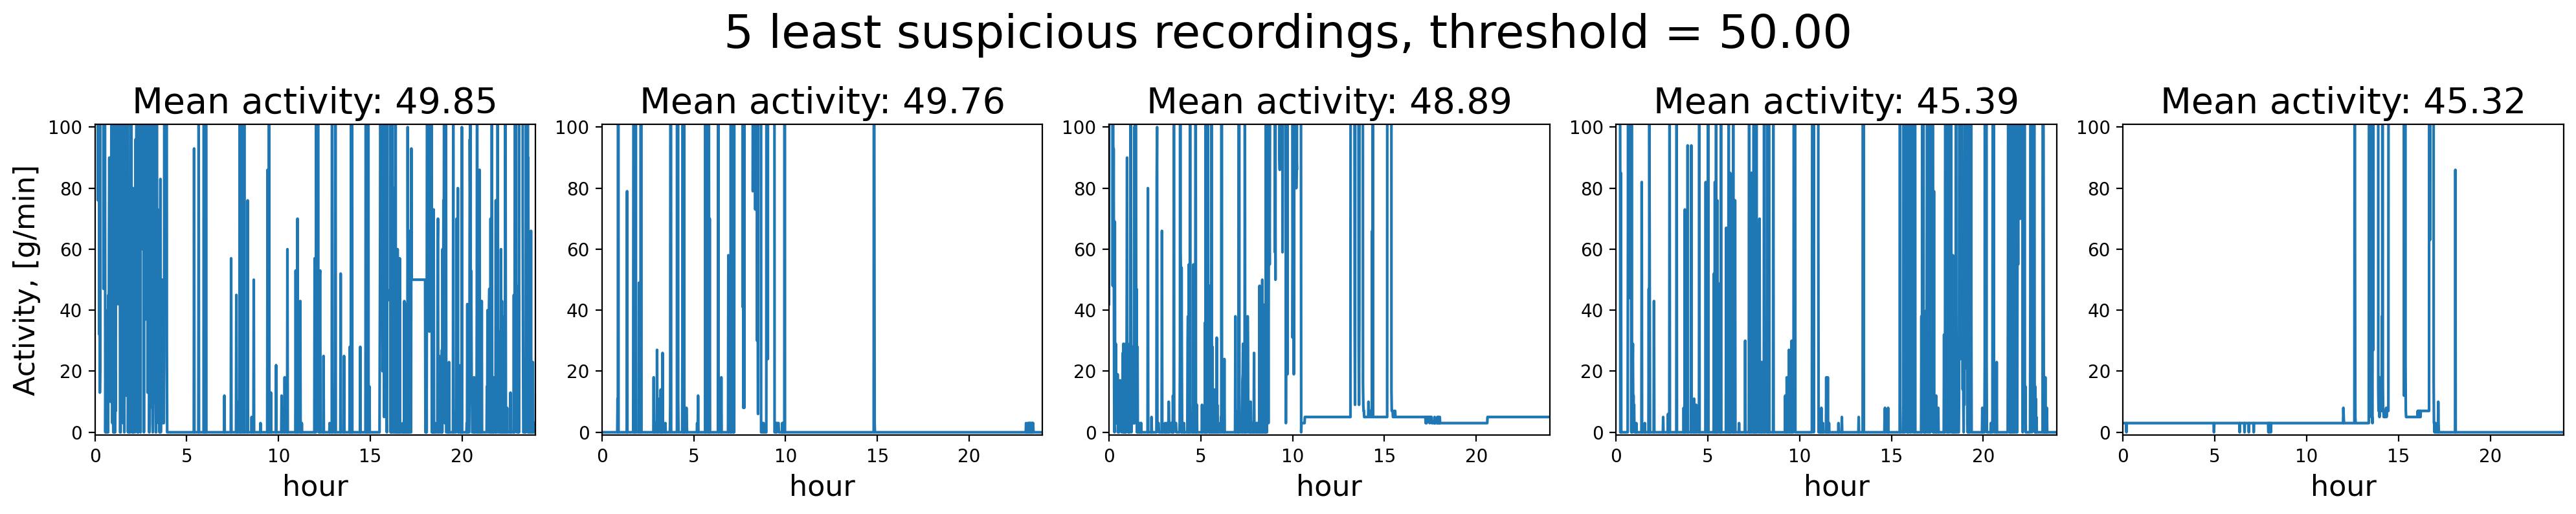
\includegraphics[width=.99\textwidth]{images/not_sus.png}
    \captionsetup{justification=centering}
    \caption{\textit{Comparison between days with suspiciously low activity to organic records of low-activity days. The top figure visualizes the least suspicious records according to the activity threshold eventually used for filtering. The bottom  figure depicts records of days with comparatively low activity, but ones that raises little suspicion. The y-axis limits were fixed for ease of comparative visual analysis.}}
    \label{fig:sus}
\end{figure}


\subsection{Feature engineering}

An important additional feature we computed for the our experiment is the dynamic of change between the two MADRS scorings. For each patient, we computed this metric as the difference between the second and first MADRS scorings divided by the duration of the observation, representing the projected average daily change of the score. The MADRS score is designed to be sensitive to changes, as it was originally developed for evaluating response to treatment, which makes the MADRS dynamic a meaningful approximation of the changes in the patient's condition. 

Exploration of the MADRS scores revealed that the vast majority of the condition subjects showed improvement over the duration of the study. The significant imbalance between the number of patients whose condition improved and the number of those who exhibited worsening symptoms poses significant challenges for the analysis implications of which will be discussed in the Discussion section of the report. Figure \ref{fig:madrs} summarises the distribution of the scores and the newly computed dynamic.

Some of the experiments required the activity data aggregated into daily readings. For this purpose, the actigraph readings were rearranged according to the patient that wore the device and the date of the recording. The resulting collections of data were then represented as numeric vectors of length at most 1440, corresponding to the number of minutes in a day. This representation of the readings was convenient for calculating and visualizing average daily activity of individual subjects and groups of subjects.

\begin{figure}[!h]
    \centering
    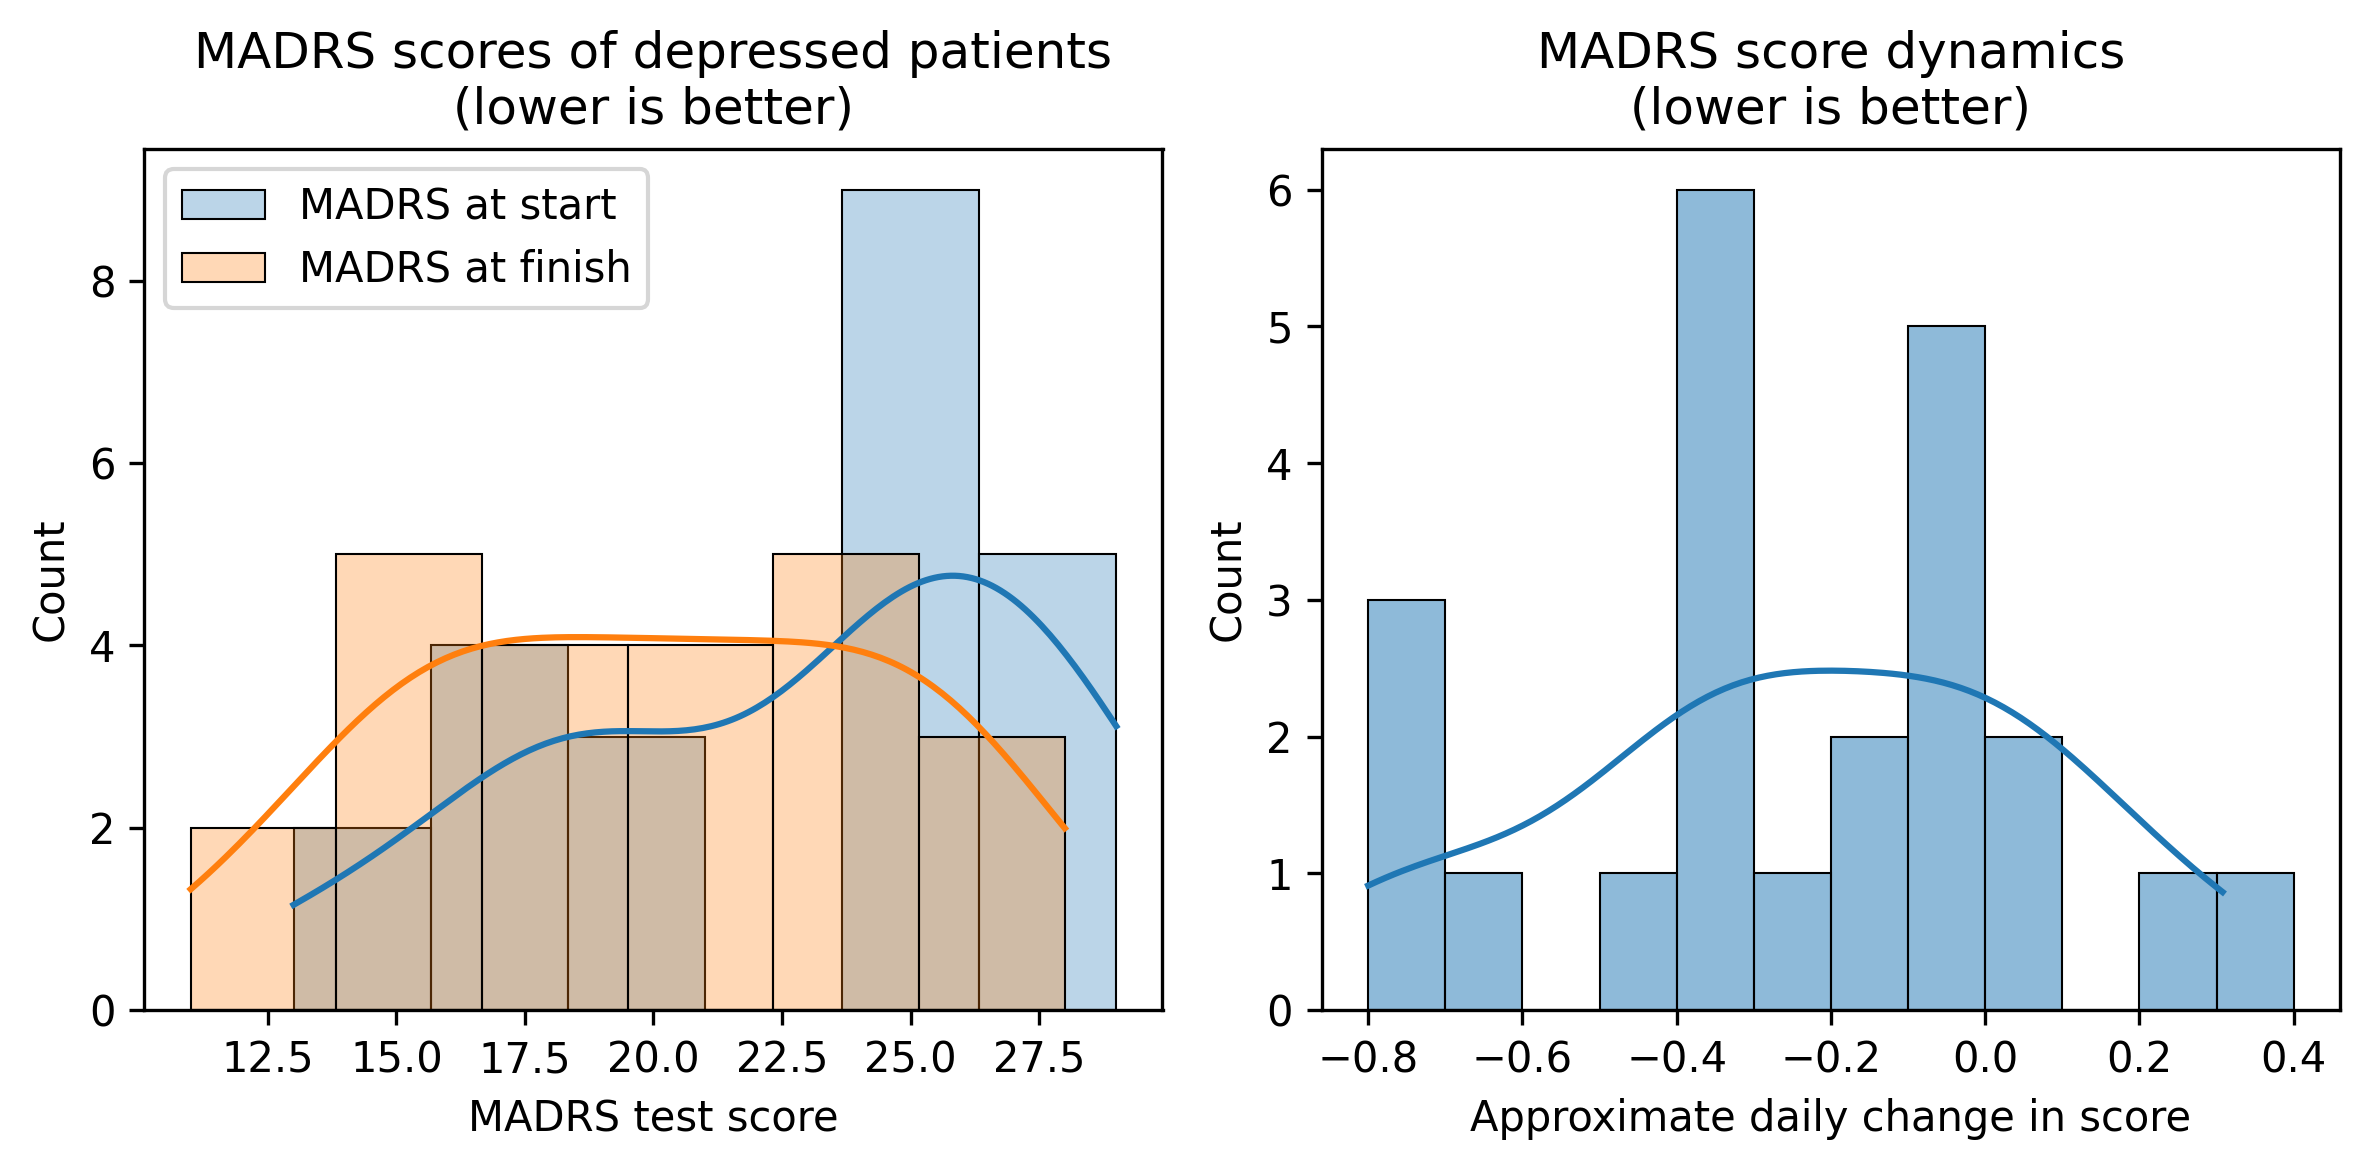
\includegraphics[width=.99\textwidth]{images/madrs.png}
    \captionsetup{justification=centering}
    \caption{\textit{Histogram of the MADRS scores reported in the data and the distribution of the computed MADRS dynamics metric.}}
    \label{fig:madrs}
\end{figure}

\section{Methods}

In the following passage we describe and motivate the methods and techniques we applied to the data set to address the goals of the project.

\subsection{Statistical analysis}

To verify a statistically significant difference between the mean daily activity among the control and condition groups, we conducted a statistical test with the null hypothesis postulating that the mean activity of the two populations are equal. Based on a visual evaluation, the activity distributions of the two subject groups complied with assumptions of normality and equal variance, hence we used an independent t-test \parencite{student1908probable} to assess the validity of the null hypothesis.

\subsection{Group level exploration}

To enable exploration of physical activity of subjects beyond comparing the entire condition group to the control group, we divided the condition group into two smaller subgroups based on the MADRS dynamic metric. The first subgroup encompassed patients who showed lowered scores (corresponding to reducing symptoms), while the second subgroup contained patients with worsening symptoms and correspondingly increasing scores. Adding a third subgroup for patients with small changes in the score was also considered, but ultimately this idea was rejected due to a limited size of the data set. For each of the two subgroups, we computed the mean and standard deviation of activity for every minute of the day.

We then proceeded to visualize the daily activity values. To eliminate high-frequency fluctuations, a moving average filter was applied with the window length of 60 minutes. Additionally, we conducted similar analysis for female subjects only, motivated by a large proportion of female patients among those who experienced worsening symptoms.

To further study the physical activity behavior of the different groups, we separated the day into four intervals — night from 0:00 to 6:00, morning from 6:00 to 12:00, afternoon from 12:00 to 18:00, and evening from 18:00 to 0:00. We visualized the mean activity distributions during each of the intervals across the studied groups using violin plots. In addition, we plotted a projection of the resulting 4-dimensional vectors onto the 2D plane by discarding the night and evening data. The choice of retained features was based on how well the features separate the different groups and how correlated they are with other features.

\section{Results}

This section details the outcomes of the experimental methods described above and presents visualizations.

\subsection{Statistical conclusions}

Through statistical testing, we were able to reject the null hypothesis (p-value of $3.62 * 10^{-5}$), meaning that there exists a statistically significant difference between mean daily physical activities of those suffering from depression and those that do not. A visualization of the activity of condition vs. control groups is presented in Figure \ref{fig:act_violin} which illustrates the suitability of the independent t-test assumptions and demonstrates the reduced activity among depressed subjects. These results are consistent with conclusions of previous studies, which identify an inverse correlation between motor activity and expression of depressive symptoms \parencite{O_Brien, Pinto, Harris}. 

\begin{figure}[!ht]
    \centering
    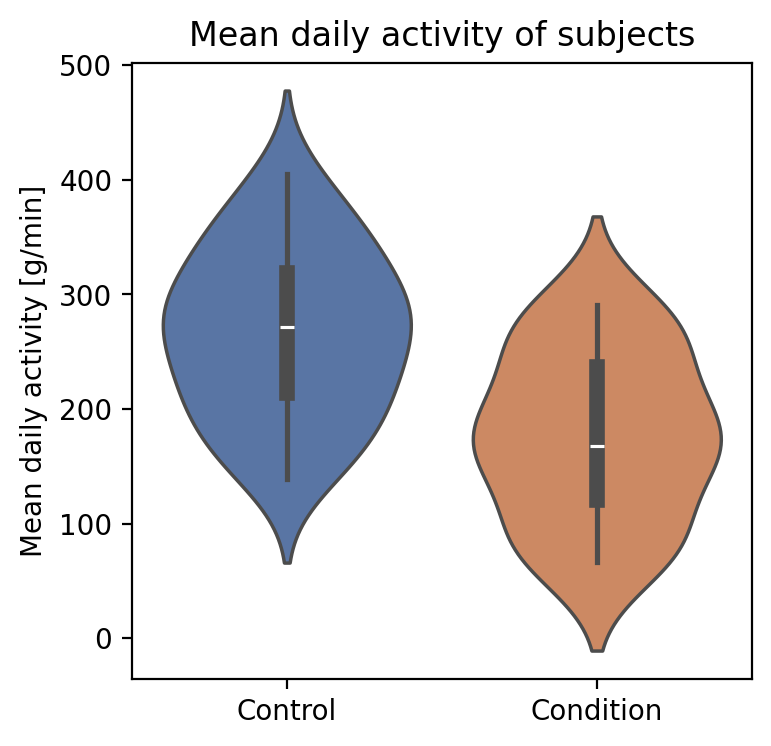
\includegraphics[width=.5\textwidth]{images/act_violin.png}
    \captionsetup{justification=centering}
    \caption{\textit{Mean daily activity of the study subjects.}}
    \label{fig:act_violin}
\end{figure}

\subsection{Exploratory findings}

Visualization of mean activity throughout the day for the three examined subgroups (Figure \ref{fig:daily_act_agg}) further clarifies how the activity of depression patients differs from that of the control group. 

\begin{figure}[!t]
    \centering
    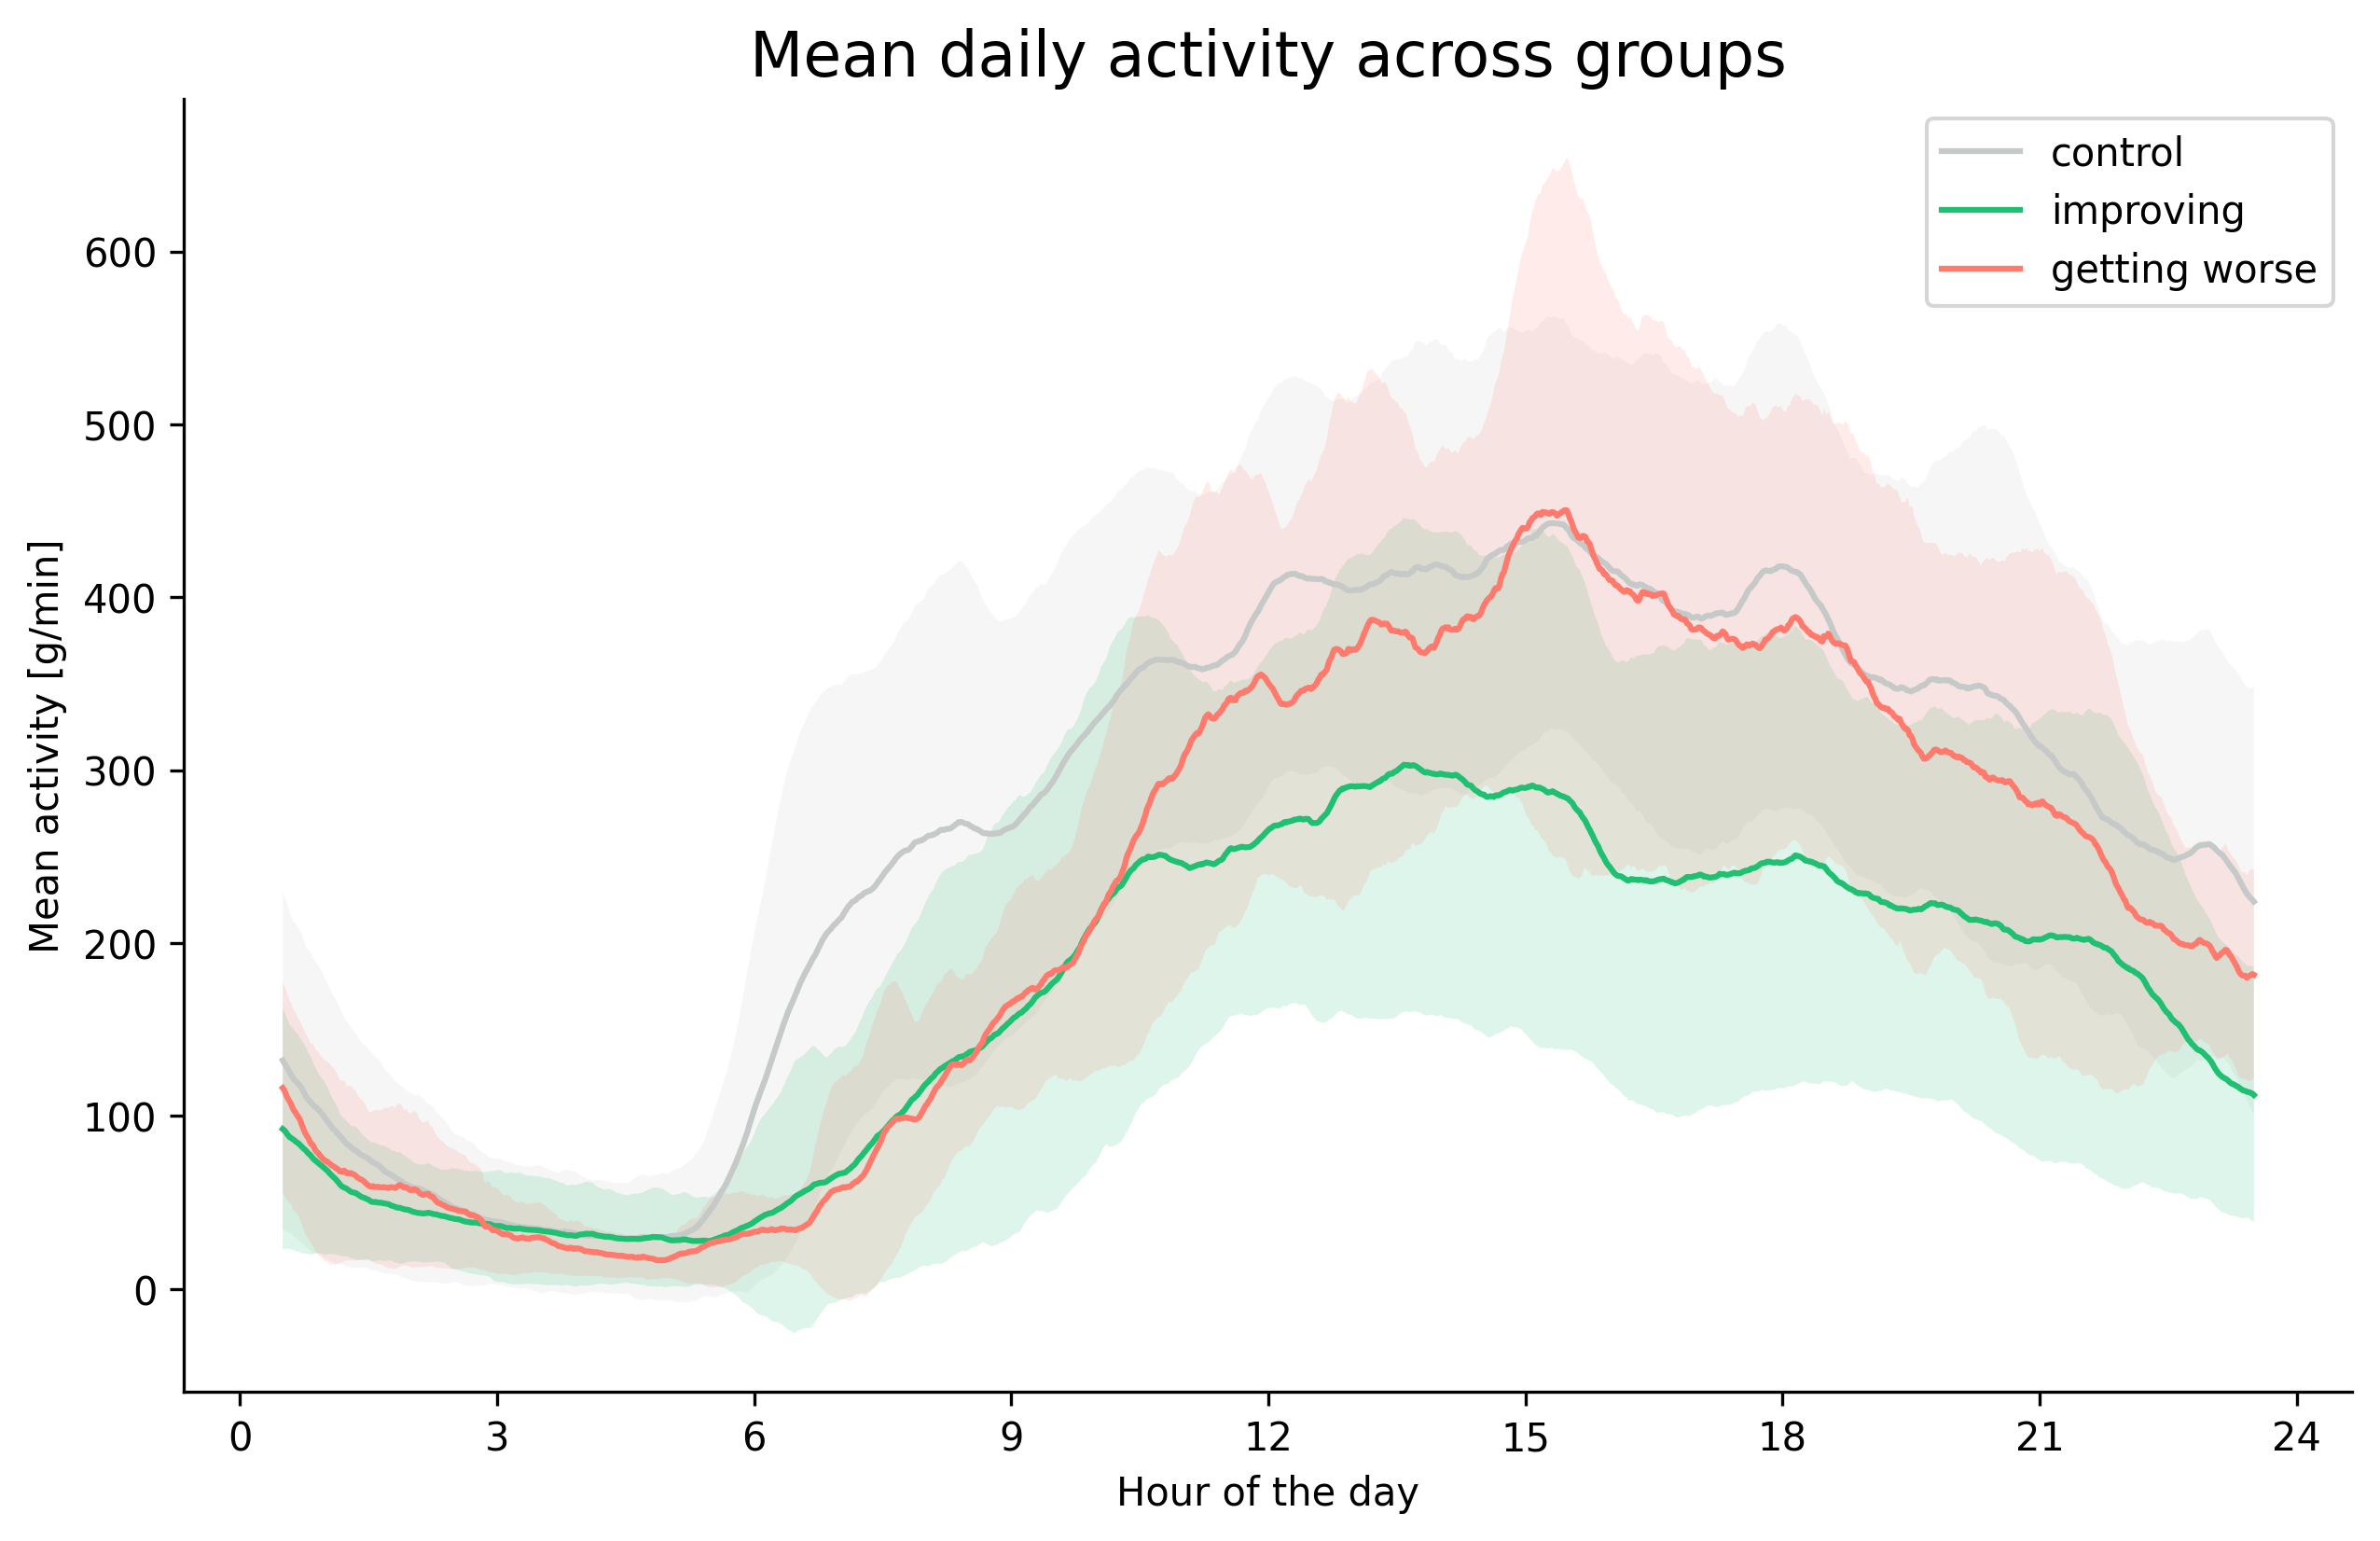
\includegraphics[width=.75\textwidth]{images/mean_act_agg.png}
    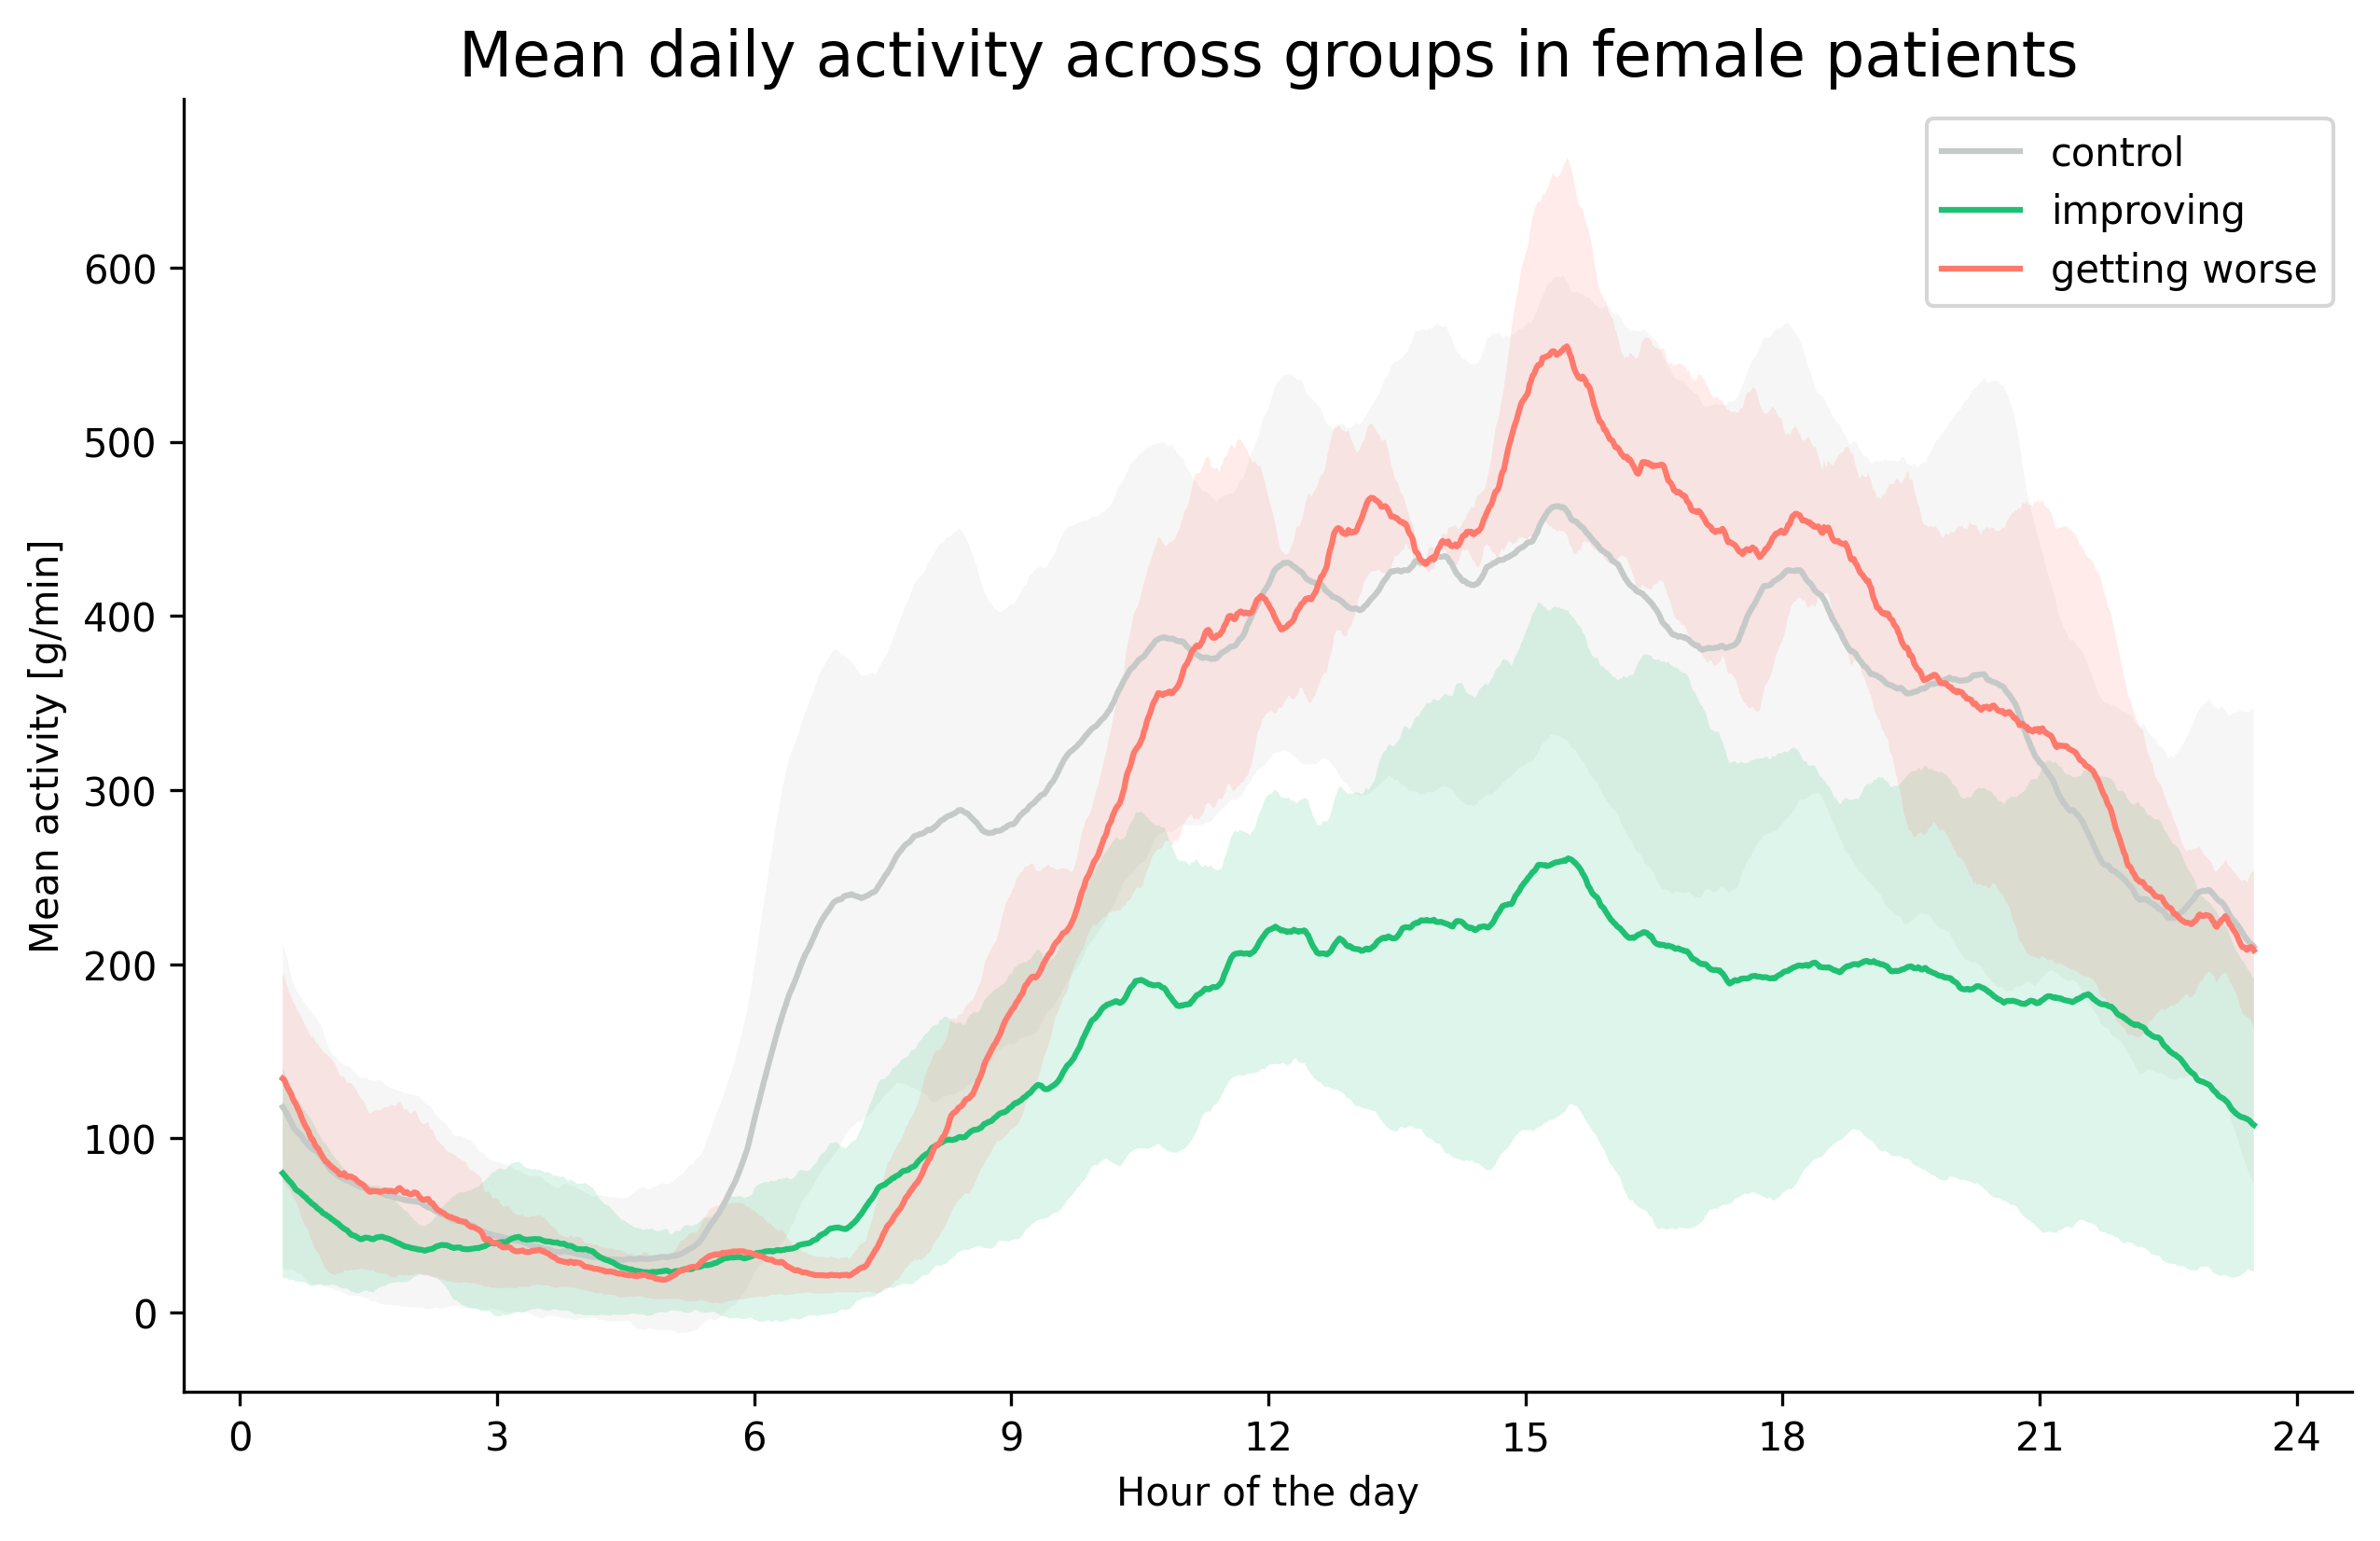
\includegraphics[width=.75\textwidth]{images/mean_act_agg_fe.png}
    \captionsetup{justification=centering}
    \caption{\textit{Mean activity throughout the day among the examined subgroups. Shaded areas represent the standard deviation range.}}
    \label{fig:daily_act_agg}
\end{figure}

We can observe that the nighttime activity between the groups is fairly consistent, but starting around 6:00 am the activity lines begin to diverge, with the lines corresponding to the condition group remaining steadily low for noticeably longer and climbing at a slower rate throughout the morning. Around 11:00 am, the lines corresponding to the two subgroups of the condition cohort sharply separate, with the activity of the improved subgroup settling at consistently lower level than the activity of control subjects through the rest of the day, while activity of patients with progressing symptoms remains much closer to the control group activity through afternoon and evening. This effect appears even more pronounced among female patients.

We can illuminate this pattern from a different perspective by examining the activity distributions for separate parts of the day, which are presented in Figure \ref{fig:act_pod}. Here we once again observe that during nights the three groups exhibit similar activity levels, in the mornings the two condition subgroups behave similarly while the control group activity increases, and in the afternoons and evenings the subgroup exhibiting worsening symptoms behave much more like the control group than the other patients.

\begin{figure}[!t]
    \centering
    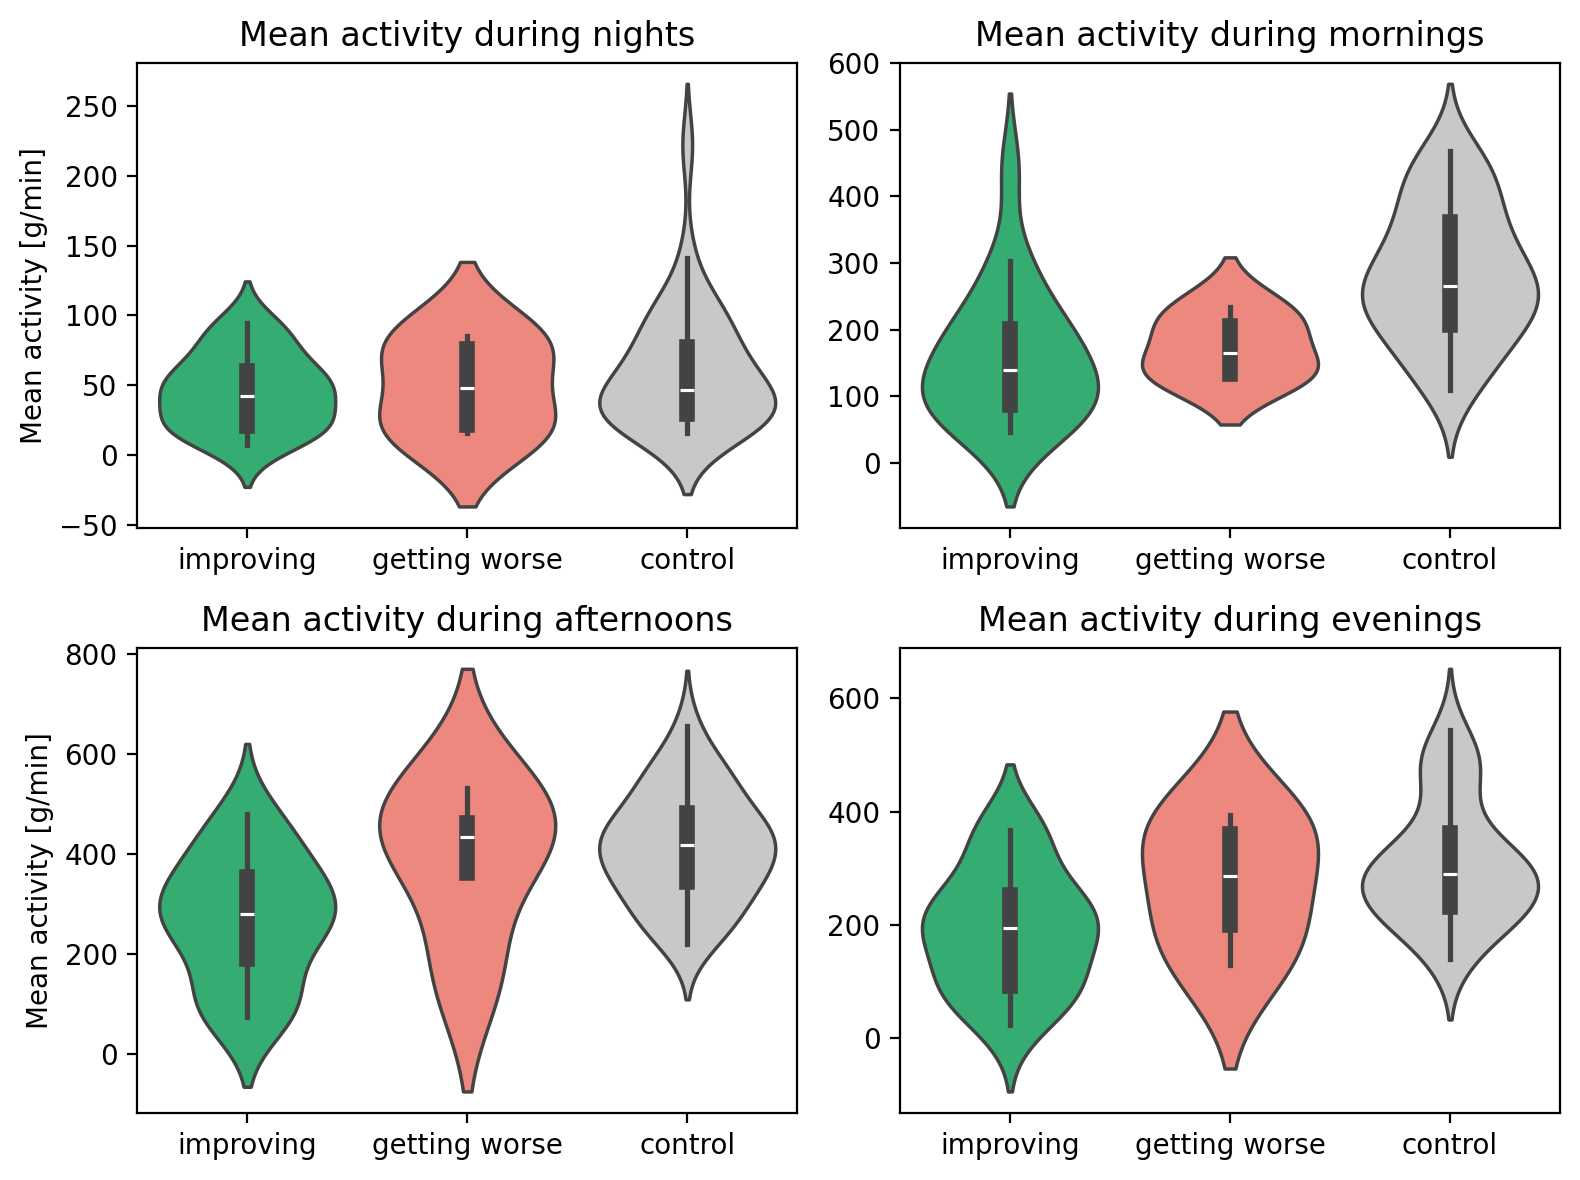
\includegraphics[width=.9\textwidth]{images/act_pod.png}
    \captionsetup{justification=centering}
    \caption{\textit{Distributions of mean physical activity during different parts of the day across studied groups.}}
    \label{fig:act_pod}
\end{figure}



Based on the time of day activity distributions, we elected to retain the morning and the afternoon activity data for the 2D plot, as the night activity provides comparatively little group separation, and the evening activity turned out to be strongly correlated with afternoon activity. The resulting embedding is presented in Figure \ref{fig:2d_act}. Here we can observe that most of the patients with progressing symptoms are localized to the upper left quadrant of the plot, with the female patients from this subgroup being entirely linearly separable from the remaining female patients with depression.

\begin{figure}[!t]
    \centering
    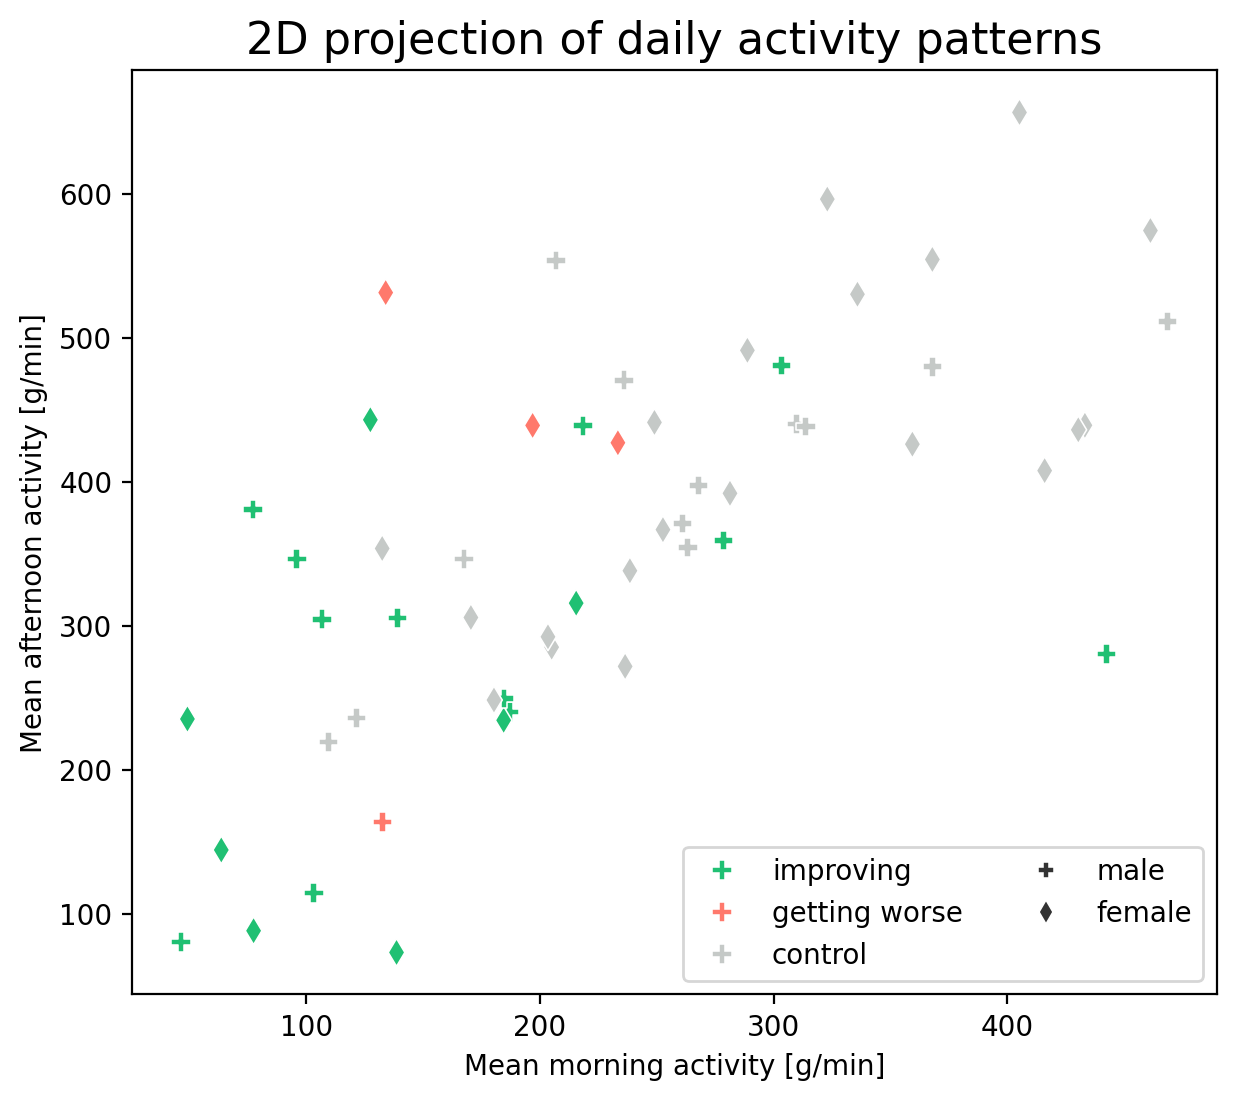
\includegraphics[width=.99\textwidth]{images/2d_act.png}
    \captionsetup{justification=centering}
    \caption{\textit{Distributions of mean physical activity during different parts of the day across studied groups.}}
    \label{fig:2d_act}
\end{figure}



\section{Conclusion and Discussion}

% In this section we summarize our findings and discusses their implications. We also present the limitations of the experimental process and conclude with a discussion on possible avenues of future work. 

% \subsection{Key findings}

% The data we examined for this project not only reaffirms the value of the actigraph as an accessible and non-invasive instrument in psychiatric diagnosis, but also supports the idea of utilizing actigraphy in monitoring the condition of already diagnosed patients. 

% \subsection{Implications of the results}

The patterns in physical activity of patients with worsening symptoms are somewhat surprising. It might seem intuitive to assume that as patients start to feel better, they tend to behave more like the healthy individuals. This intuition poses a risk of mistaking partially normalizing activity patterns for signs of recovery, both from the psychiatrist perspective and, crucially, from the point of view of the patient. Such errors could lead to decisions that only exacerbate the disorder, such as discontinuing medication. The potential for error highlights the importance of objective methods for movement measurement as well as careful further research into movement features that might be associated with a worsening mental condition.

Our experiments suggest that a combination of reduced activity in the morning with normal activity during the rest of the day could be one such feature. While it is difficult to speculate on the mechanism of such an association, one hypothesis we do put forward is that some depressed people who are forced or convinced to operate at consistently elevated levels of activity could be seeing their symptoms ultimately worsen. The highly limited number of patients with increasing MADRS score in the studied data set leaves this line of reasoning as only a hypothesis, since confirming or rejecting it would necessitate a larger or more balanced study. With a more substantial amount of data, it would also be possible to investigate the possibility of developing an automatic system for indicating worsening patient symptoms through the application of machine learning techniques.

Besides the uncertainty induced by the limited size of the subgroup of interest, we also need to consider the reliability of the metric used to identify patients with worsening symptoms. The data used for the present study only offered two Montgomery-Asberg Depression Rating Scale scorings for each patient. While the scale is designed to be sensitive to changes in the patient's condition, some of the variance between two assessments could be introduced by temporary fluctuations of the patient's condition, thus obscuring the true trend of disorder progression. If a new actigraphy study were to be considered, it might be sensible to design the experiment with the need for more robust assessment methods in mind, be that through longer study duration or additional sources of information on the subject's condition.



\newpage
\printbibliography

\end{document}
